\setcounter{section}{5}
\section{Stabilität von linearen Systemen}
\begin{tcolorbox}[colback=white!10!white,colframe=green!30!black,title=Stabilität] 
Alle Pole der Übertragungsfunktion müssen in der LHE sein. \textbf{Steuerung} stabilisiert nicht. 
\textbf{Regelung:}

    \begin{figure}[H]
        \centering
        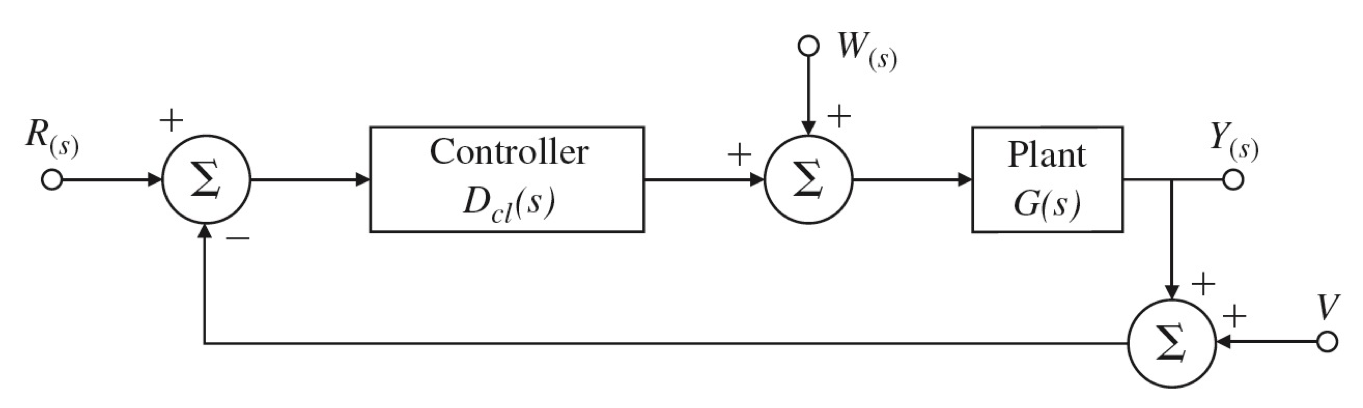
\includegraphics[width=.7\textwidth]{images/regler}
\end{figure}
    \begin{align*}
    &G(s) = \frac{b(s)}{a(s)}  && D_{OL} = \frac{c(s)}{d(s)}
    &1+ G D_{CL} = 0\\ 
    &1 + \frac{bc}{ad} = 0  &&
    a(s)d(s) + b(s)c(s) = 0 
    \end{align*}
Die Regelung reduziert die Auswirkung von Störung um $1+ AK$
\end{tcolorbox}

%ROUTH-Criterion
\subsection{Routh-Stabilitätskritetium}
\begin{tcolorbox}[colback=white!10!white,colframe=green!30!black,title=Routh Kriterium] 
    Gibt Aussage darüber, ob alle Pole des charakteristischen Polynoms $P(s)$ in der LHE liegen:
    \begin{align*}
        P(s) = s^n + a_1s^{n-1}+a_2s^{n-2}+\ldots + a_{n-1}s+a_n
    \end{align*}
    Es muss gelten $a_i > 0$ für $\forall i \in \mathrm{N}$
    \begin{align*}
        \begin{matrix}[0.6]
        n & s^n & 1 & a_2 & a_4 & \ldots \\
        n-1 & s^{n-1} & a_1 & a_3 & a_5 & \ldots \\
        n-2 & s^{n-2} & b_1 & b_2 & b_3 & \ldots \\        
        n-3 & s^{n-3} & c_1 & c_2 & c_3 & \ldots \\
        \vdots & \vdots & \vdots & \vdots & \vdots  \\
        2 & s^2 & * & *  \\
        1 & s^1 & * \\
        0 & s^0 & \ldots
        \end{matrix}
    \end{align*}
    Die Koeffizienten werden folgendermaßen errechnet:
    \begin{align*}
        & b_1 = -\frac{\begin{vmatrix}
            1 & a_2 \\ a_1 & a_3
            \end{vmatrix}}{a_1} = \frac{a_1a_2-a_3}{a_1} & c_1 = -\frac{\begin{vmatrix}
            a_1 & a_3 \\ b_1 & b_2
            \end{vmatrix}}{b_1} = \frac{b_1a_3-a_1b_2}{b_1}\\
        & b_2 = -\frac{\begin{vmatrix}
            1 & a_4 \\ a_1 & a_5
            \end{vmatrix}}{a_1} = \frac{a_1a_4-a_5}{a_1} & c_2 = -\frac{\begin{vmatrix}
            a_1 & a_5 \\ b_1 & b_3
            \end{vmatrix}}{b_1} = \frac{b_1a_5-a_1b_3}{b_1}\\
        & b_3 = -\frac{\begin{vmatrix}
            1 & a_6 \\ a_1 & a_7
            \end{vmatrix}}{a_1} = \frac{a_1a_6-a_7}{a_1} & c_3 = -\frac{\begin{vmatrix}
            a_1 & a_7 \\ b_1 & b_4
            \end{vmatrix}}{b_1} = \frac{b_1a_7-a_1b_4}{b_1}
    \end{align*}
    
    \begin{itemize}
        \item Alle Elemente der ersten Spalte positiv $\Rightarrow$ Wurzeln in der offenen LHE                
        \item $\#$-Wurzeln  in der geschlossenen RHE   = $\#$-Vorzeichenwechsel 
        \item Wenn das erste Element einer Zeile null ist, setze $\epsilon > 0$. Stabilitätskriterium für $\epsilon \rightarrow 0_+$
    \end{itemize}
\end{tcolorbox}


\begin{tcolorbox}[colback=white!10!white,colframe=green!30!black,title=Sensitivität] 
    Sensitivität beschreibt die Reaktion des Systems auf Änderung im Parameter
    \begin{align*}
        & S_{A}^{T_{CL}} = \frac{A}{T_{CL}}\frac{d T_{CL}}{dA}
        & |S_{G}^{T_{CL}}| = \frac{1}{1+G(i\omega_0)D(i\omega_0)}
        \end{align*}
    \begin{align*}
        &T_{CL} -\text{ Closed-Loop Übertragungsfunktion} & A - \text{Parameter}
    \end{align*}
\end{tcolorbox}
%CLM-Criterion
\subsection{CLM-Stabilitätskriterium}
\begin{tcolorbox}[colback=white!10!white,colframe=green!30!black,title=CLM Kriterium] 
    \textbf{Annahme:}
    $m$-Wurzeln in RHE  und $n-m$-Wurzeln ($n \leq m$)
    
    Charakteristische Gleichung:
    \begin{align*}
        P(s) = a_0 + a_1s + a_2s^2 + \ldots + a_n s^n = 0 
    \end{align*}
    Einsetzen $s = j\omega$. 
    Das System ist dann asymptotisch stabil, wenn
    \begin{enumerate}
        \item die Ortskurve $P(j\omega)$  für $0 \leq \omega \leq \infty$ die Quadranten abwechselnd durchläuft (sich die Nullstellen des Real und Imaginärteils von $P(j\omega) = U(\omega)+iV(\omega)$ abwechseln.) 
        \item Real- und Imaginärteil zusammen $n$ (Grad der Gleichung) reelle Nullstellen im Bereich $0 \leq \omega \leq \infty$ besitzen 
    \end{enumerate} 
    
    
    
    
    \tcblower
    
    \textbf{Beispiel:}
    \begin{align*}
        &P(s) = 2 + 5s +7s^2 +8s^3 +4s^4 +s^5\\
        &P(j\omega) = 2 + 5j\omega + 7(j\omega)^2 +8 (j\omega)^3 + 4 (j\omega)^4 + (j\omega)^5\\
        &2-7\omega^2 +4\omega^4 + j (5\omega - 8\omega^3 +\omega^5)\\
        &U(\omega) + jV(\omega)
    \end{align*}
    Realteil hat die Nullstellen:
    \begin{align*}
        &2-7\omega^2 +4\omega^4 = 0 \\
        &\omega_1^2 = 0,36 & \omega_2^2= 1,39
    \end{align*}
        Imaginärteil hat die Nullstellen:
        \begin{align*}
        &5\omega - 8\omega^3 +\omega^5= 0 \\
        &\omega3 = 0  & \omega_4^2= 0,68 & & \omega_5^2= 7,32 
        \end{align*}
        
        Insgesamt sind $n=5$ reelle Nullstellen mit $\omega_i >= 0$. Diese wechseln sich jeweils ab, damit ist das System asymptotisch stabil. $\omega_3 < \omega_1 < \omega_4 < \omega_2 < \omega_5$ Siehe Grafik:
        \begin{figure}[H]
\centering
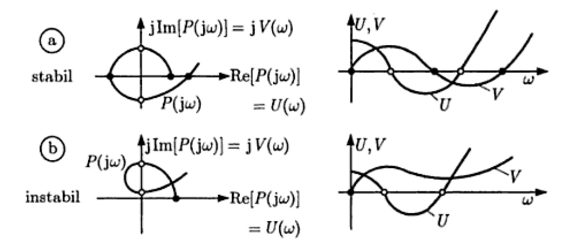
\includegraphics[width=0.7\linewidth]{images/clm}
\label{fig:clm}
\end{figure}

        
\end{tcolorbox}

